\documentclass[brazil]{article}
\usepackage{ae,aecompl}
\usepackage[T1]{fontenc}
\usepackage[utf8]{inputenc}
\usepackage[a4paper]{geometry}
\geometry{verbose,lmargin=3cm,rmargin=3cm}
\setcounter{tocdepth}{0}
\usepackage{amsmath}
\usepackage{caption}
\usepackage{float}
\usepackage{graphicx}
\usepackage{amssymb}
\usepackage{verbatim} % comentarios


\makeatletter
%-%-%-%-%-%-%-%-%-%-%-%-%-%-%-%-%-%-%-%-%-%-%-%-%-%
% EE531: laboratório de Eletrônica Básica I       %  
% Experimento 2: Diodos                           %
% Data:20/08/2010                                 %
% Unicamp,Campinas,São Paulo,Brasil               % 
% Grupo:                                          %
%       - Daniel Lins Mattos                      %
%       - Raquel Mayumi Kawamoto                  %
%       - Tiago Chedraoui Silva                   % 
%-%-%-%-%-%-%-%-%-%-%-%-%-%-%-%-%-%-%-%-%-%-%-%-%-%
%\documentclass[letter]{article}  % formato impressao IC
% formato impressao FEEC

%%% fontes %%%
% dá suporte para os termos na língua portuguesa do Brasi
% acentuação
\usepackage{ae}\usepackage{aecompl}\usepackage{aeguill}% pdfs mais bonitos =)

%%% outros %%%
\usepackage{multirow}\@ifundefined{definecolor}
 {\usepackage{color}}{}
\usepackage{indentfirst}% retira padrao americano de paragrafos
\usepackage{multicol}\usepackage[linkbordercolor={1 1 1},urlcolor=black,colorlinks=true]{hyperref}% links
\usepackage{subfig}

% circuito eletrico
\usepackage{electComp}\usetikzlibrary{decorations,decorations.pathmorphing,decorations.pathreplacing}
\usepackage{pstricks}\usepackage{boxdims}



\renewcommand{\thefigure}{\arabic{figure}}

\date{Novembro 12, 2010}
% Capa estilizada %
\newcommand*{\titleTMB}{\begingroup \centering \settowidth{\unitlength}{\LARGE EE531} {\large\scshape EE531 - Turma S}\\[0.2\baselineskip] \rule{11.0cm}{1.6pt}\vspace*{-\baselineskip}\vspace*{2pt} \rule{11.0cm}{0.4pt}\\[\baselineskip] {\LARGE  Amplificador operacional \\ com realimentação negativa}\\\vspace*{\baselineskip}  {\itshape Laboratório de Eletrônica Básica V - Segundo Semestre de 2010}\\ \rule{11.0cm}{0.4pt}\vspace*{-\baselineskip}\vspace{3.2pt} \rule{11.0cm}{1.6pt}\\[\baselineskip] {\large\scshape Professor: José Cândido Silveira Santos Filho}\par \vfill {\normalsize   \scshape 
    \begin{center} 
      \begin{tabular}{  l  l  p{5cm} } 
 	Daniel Lins Mattos & RA: 059915\\
        Raquel Mayumi Kawamoto & RA: 086003\\
        Tiago Chedraoui Silva  & RA: 082941\\
      \end{tabular} \end{center}
    \itshape 1 de outubro de 2010    }\\[\baselineskip] \vspace{3.2pt} \endgroup}

\makeatother

\usepackage{babel}

\begin{document}
\titleTMB \newpage{}


Este experimento visa o estudo do  amplificador operacional em circuito integrado LM741, que é um dos amplificadores comerciais mais populares.
Um desenho da função de cada pino do integrado é apresentado na figura \ref{circ:1} e sua descrição é apresentada na tabela a seguir:

\begin{table}[H]
\begin{center}
\caption{Descrição dos pinos de um LM741}
\begin{tabular}{cp{10cm}}
\hline 
Pino & Descrição\tabularnewline
\hline
\hline 
1 e 5 & Offset - Os pinos 1 e 5 costumam ser conectados a um resitor variável, juntamente com a entrada negativa da alimentação, buscando equilibrar as tensões da entrada.\tabularnewline
\hline 
2 & Entrada inversora do amplificador ($V_-$) \tabularnewline
\hline 
3 & Entrada não inversora do amplificador ($V_+$)\tabularnewline
\hline 
4 & Alimentação Negativa ($V_{s-}$)\tabularnewline
\hline 
6 & Tensão de saída\tabularnewline
\hline 
7 & Alimentação positiva ($V_{s-}$)\tabularnewline
\hline 
8 & Não conectado\tabularnewline
\hline
\end{tabular}
\end{center}
\end{table}

\begin{comment}
\begin{itemize}
       \item Off-set - o pino 1 e o pino 5 costumam ser conectados a um resitor variável, juntamente com a entrada negativa da alimentação, buscando equilibrar as tensões da entrada.
       \item Entrada inversora.
       \item Entrada não inversora.
       \item Alimentação negativa
       \item Outro pino do off-set.
       \item Tensão de saída.
       \item Alimentação positiva.
       \item Não conectado.
\end{itemize}
\end{comment}

\vspace{3mm}
\begin{figure}[h]
\centerline{\input circ1.tex}
\caption{Pinos de saída de um 741 \label{circ:1}}
\end{figure}


Assim como nos demais experimentos anteriores, foi utilizado o protoboard para a montagem dos circuitos. E os principais componentes utilizados foram dois CI LM741, um trimpot 20 voltas de 10$k\Omega$ e resistores  de 1$k\Omega$, 10$k\Omega$, 20$k\Omega$ e 200$k\Omega$. 



\section*{Parte experimental}

\section*{3.1}
Inicialmente, o circuito da figura \ref{circ:4} é montado e é aplicado um sinal senoidal na entrada cuja amplitude é a menor possível e sua frequência vale 100 Hz. A partir dessa configuração, o gráfico representando a saída é apresentado na figura \ref{3.1}.

\vspace{3mm}
\begin{figure}[h]
\centerline{\input circ4.tex}
\caption{Amplificador operacional em malha aberta \label{circ:4}}
\end{figure}


\begin{figure}[H]
\begin{centering}
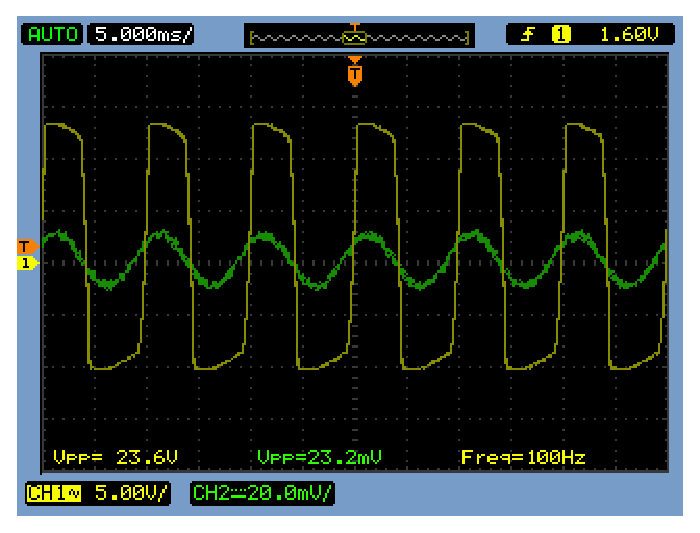
\includegraphics[scale=0.5]{figuras/31bck}
\caption{Onda de saída do circuito da figura \ref{circ:4} \label{3.1}}
\par\end{centering}
\end{figure}


 É possível concluir, observando as curvas de saída, que no amplificador operacional a tensão de saída fica limitada ao intervalo de -12 V a +12 V. Isso já era esperado. Esse fato leva a uma onda praticamente quadrada na saída, para um ganho A muito elevado. No caso da nossa equipe, isso não ocorreu perfeitamente, provavelmente devido a desbalanceamentos no AMP-OP, ou problemas na montagem do circuito.





\newpage
\section*{3.3}

\begin{eqnarray*}
V_+=V_{in}\\
V_-=BV_{out}
 \end{eqnarray*}

\vspace{-8mm}

\begin{align*}
V_{out}& =  A(V_+-V_-) \\
&=A(V_{in}-BV_{out})\\
&=AV_{in}-ABV_{out}
\end{align*}

\vspace{-5mm}
\[
(1+AB)V_{out}=AV_{in}
\]


\begin{equation}
\frac{V_{out}}{V_{in}}=\frac{A}{1+AB}
\label{Ganho de malha fechada A_f}
\end{equation}
\captionof*{figure}{Ganho de malha fechada $A_f$}

\begin{equation}
\lim_{A \to \infty}A_f=\lim_{A \to \infty}\frac{A}{1+AB}=\frac{1}{B}
\end{equation}

Ou seja, para valores elevados de A, o ganho de malha fechada $A_f$ é facilmente controlável pelo fator de realimentação B. Para B>1, $A_f<A$. Quer dizer, o ganho de malha fechada pode ser feito menor que o ganho de malha aberta. 



\section*{3.4}

\begin{eqnarray*}
V_-=BV_{out}=V_{out}\rightarrow B=1\\
A_f=A_{v}=\frac{A}{1+A.1} \approxeq 1\;\;\; \text{para}\;\;\;A\gg1
 \end{eqnarray*}
Ou seja, é um Buffer.


\begin{figure}[h!]
\centerline{\input circ3.tex}
\caption{Circuito Buffer \label{circ:3}}
\end{figure}


\section*{3.5}
 Posteriormente, o circuito da figura \ref{circ:3} é montado e, na entrada, é aplicado um sinal senoidal. Utilizando o modo X-Y do osciloscópio, o gráfico da figura \ref{3.5} é obtido.

Do gráfico obtemos um ganho $\frac{V_{out}}{V_{in}}\approxeq 1$, já que para cada volt aumentado na saída, sua entrada também aumenta em um volt.
Porém, se a entrada aumentar consideravelmente, a saída deve-se saturar em 12 Volts, perdendo, portanto, a linearidade do gráfico, que para valores de entrada maiores apresentará uma saída constante a 12 volts e para valores menores uma saída constante a -12 Volts.

\begin{figure}[H]
\begin{centering}
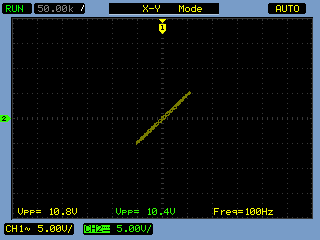
\includegraphics[scale=0.5]{figuras/35xy}
\par\end{centering}
\caption{Função de transferência $V_{in}$ x $V_{out}$ \label{3.5}}
\end{figure}



\section*{3.6}
O valor experimental do Slew Rate é aproximadamente 0,88 V/us, sendo que o valor típico do SR para um amplificador LM741A é de 0,7 V/us. O valor é satisfatoriamente próximo daquele fornecido pelo fabricante no data sheet do componente. 


\begin{figure}[H]
\begin{centering}
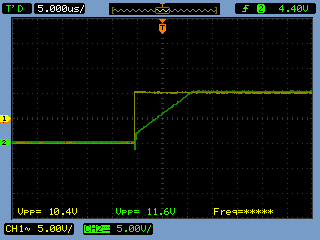
\includegraphics[scale=0.5]{figuras/36}
\par\end{centering}
\caption{}
\end{figure}


\section*{3.7}

\begin{figure}[H]
\begin{centering}
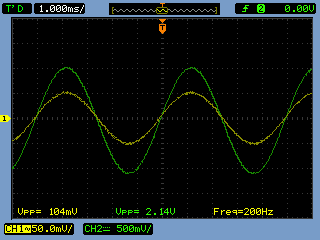
\includegraphics[scale=0.5]{figuras/37}
\par\end{centering}
\caption{}
\end{figure}
%

\section*{3.8}
Justificativa para $R=R_1\parallel R_2$


As correntes de polarização nas entradas inversora e não-inversora do AMP-OP geram uma
queda de tensão nas extremidades dos componentes do circuito, criando assim uma tensão de offset.

Se a resistência vista da entrada inversora for a mesma que a da entrada não-inversora, a queda de tensão será a mesma nessas duas extremidades, teoricamente eliminando o offset. A resistência vista da entrada inversora é  $R_1\parallel R_2$, portanto escolhe-se esse valor para R.

\begin{figure}[H]
\begin{centering}
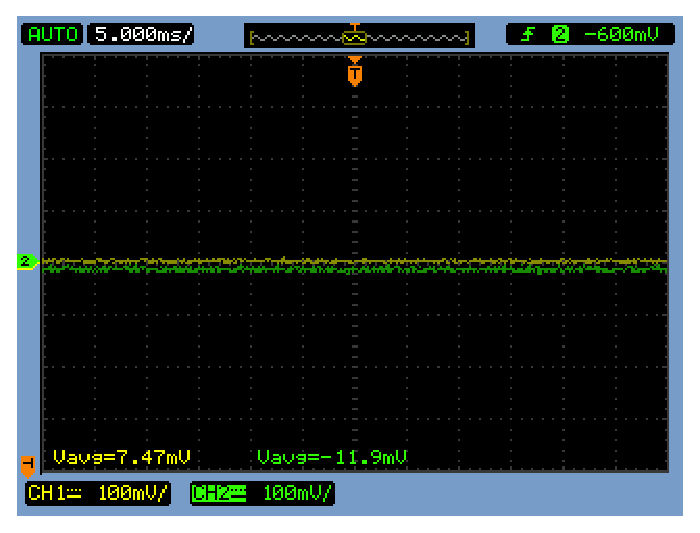
\includegraphics[scale=0.5]{figuras/382cr}
\par\end{centering}

\caption{}

\end{figure}


\begin{figure}[H]
\begin{centering}
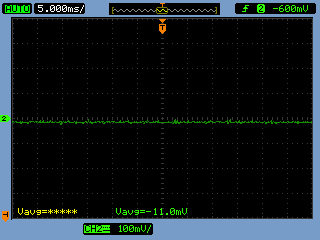
\includegraphics[scale=0.5]{figuras/382cres}
\par\end{centering}

\caption{}

\end{figure}


\section*{3.9}

Para minimizar o offset devido a desbalanceamento interno do amplificador operacional, é adicionado o potenciômetro ao circuito, resultando no circuito da figura \ref{circ:5}.

\vspace{3mm}
\begin{figure}[h!]
\centerline{\input circ5.tex}
\caption{Ajuste de offset \label{circ:5}}
\end{figure}

\begin{figure}[H]
\begin{centering}
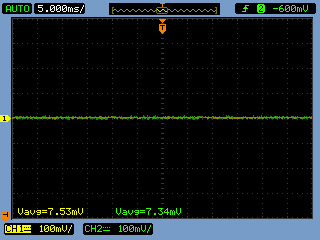
\includegraphics[scale=0.5]{figuras/39}
\par\end{centering}
\caption{}
\end{figure}



\section*{3.10}
Um circuito inversor....
Assim, para confirmar seu funcionamento, foi projetado um circuito inversor com ganho -10, conforme a figura \ref{circ:2}.
Como  $\frac{V_{out}}{V_{in}}= \frac{-R_{2}}{R_{1}}= -10$, escolheu-se, dentre os resistores fornecidos para o experimento, os valores de $R_1=1k\Omega$ e $R_2=10k\Omega$.

As ondas de entrada e saída são apresentadas no gráfico da figura \ref{3.10}, através das quais é possível ver que existe um aumento de -10, já que as fases entre saída e entrada estão diferindo em 180 graus e os valores pico a pico da saída são 10 vezes maior que o valores de entrada. 

\begin{figure}[H]
\centerline{\input circ2.tex}
\caption{Amplificador inversor\label{circ:2}}
\end{figure}


\begin{figure}[H]
\begin{centering}
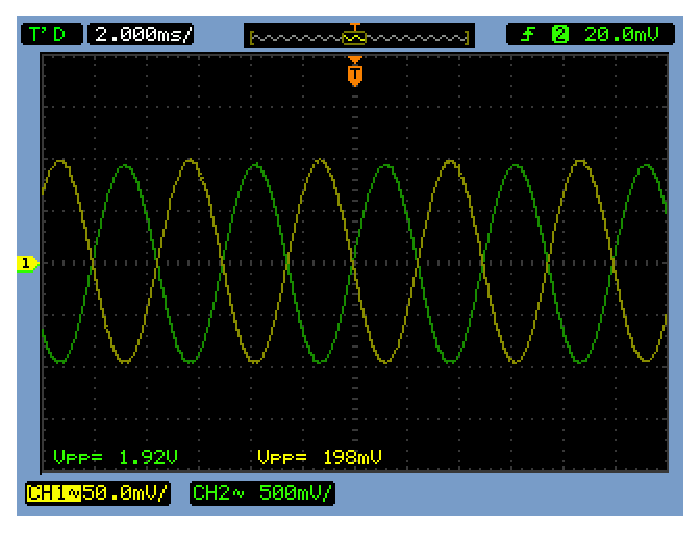
\includegraphics[scale=0.5]{figuras/310}
\par\end{centering}
\caption{Ondas de entrada e saída do circuito da figura \label{3.10}}
\end{figure}

\section*{3.11}
\begin{figure}[H]
\begin{centering}
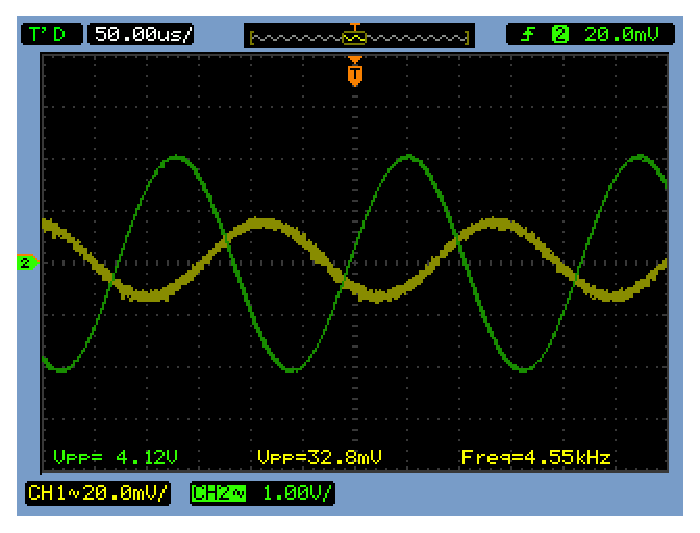
\includegraphics[scale=0.5]{figuras/311fh}
\par\end{centering}

\caption{}

\end{figure}




\end{document}
